%%%%%%%%%%%%%%%%%%%%%%%%%%%%%%%%%%%%%%%%%%%%%%%%%%%%%%%%
%%%%%%%%%%%%%%%%%%%%%%%%%%%%%%%%%%%%%%%%%%%%%%%%%%%%%%%%
\section{General Machine Learning Concepts}
\label{additional:ml:general}

%%%%%%%%%%%%%%%%%%%%%%%%%%%%%%%%%%%%%%%%%%%%%%%%%%%%%%%%
\subsection{ROC Curves}
\label{additional:ml:general:eval:ROC}
% TODO
% TODO cite in text \cref{fig:ml:roc}

\begin{figure}[H]
\centering
  \begin{subfigure}[c]{0.48\textwidth}\centering
  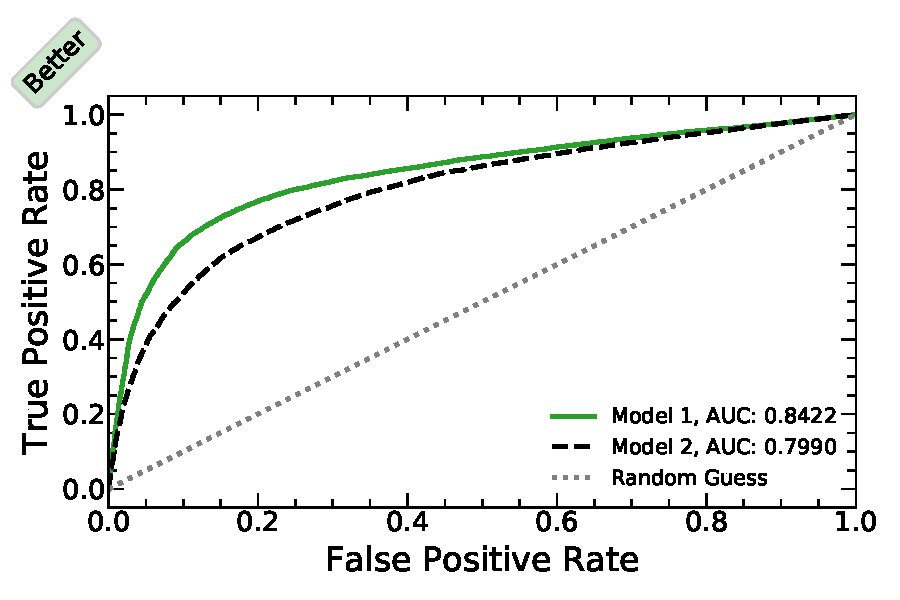
\includegraphics[width=\textwidth,trim={0.18cm 0.3cm 0.18cm 0.3cm},clip]{figures/ml/roc_curves/roc.pdf}% trim={<left> <lower> <right> <upper>}
  \caption{TPR vs FPR}
  \label{fig:ml:roc:standard}
  \end{subfigure}
  ~
  \begin{subfigure}[c]{0.48\textwidth}\centering
  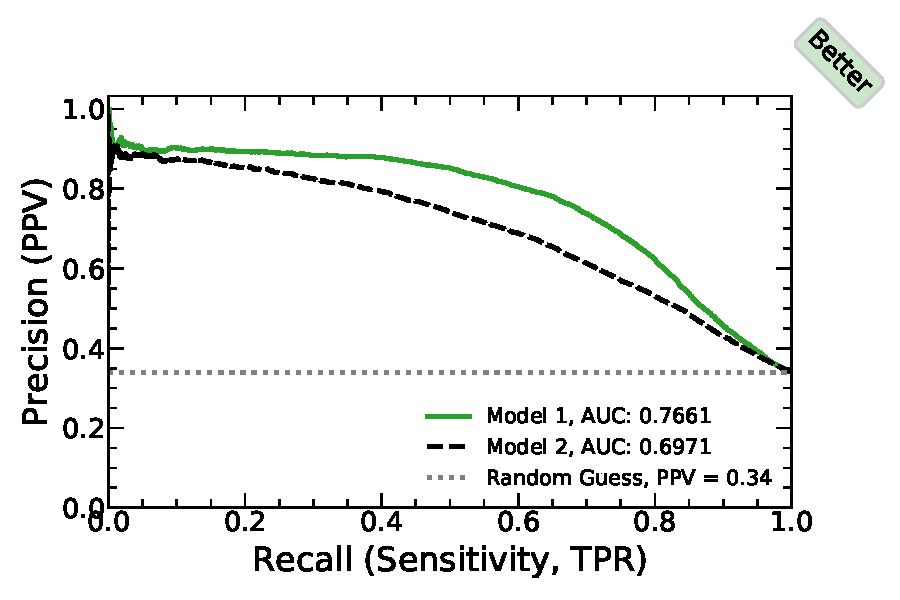
\includegraphics[width=\textwidth,trim={0.18cm 0.3cm 0.18cm 0.3cm},clip]{figures/ml/roc_curves/roc_precision_recall.pdf}% trim={<left> <lower> <right> <upper>}
  \caption{Precision vs Recall}
  \label{fig:ml:roc:precision_recall}
  \end{subfigure}
\caption{
Example ROC curves, generated by \texttt{\href{http://github.com/mepland/roc_curve_demo}{roc\_curve\_demo}}.
Note that model $1$ in solid green outperforms model $2$ when looking at TPR vs FPR and precision vs recall.
The random guess line in the precision vs recall plot is set by the class balance,
in this case the training set contained \SI{34}{\percent} signal.
}
\label{fig:ml:roc}
\end{figure}

%%%%%%%%%%%%%%%%%%%%%%%%%%%%%%%%%%%%%%%%%%%%%%%%%%%%%%%%
\subsection{Selecting a Decision Threshold}
\label{additional:ml:general:eval:decision_threshold}

% include \cref to significance section, if eventually added

In physics we may try to maximize the significance $Z$ of a classifier\footnote{And or
work with the \href{https://en.wikipedia.org/wiki/Neyman\%E2\%80\%93Pearson\_lemma}{Neyman-Pearson framework}.} by
picking an optimal point along the ROC curve to set the decision threshold.
However in data science it is often better to create a payoff matrix of the anticipated
benefits associated with a TP or TN, and costs associated with a FP or FN,
for the particular business case at hand.
The expected value of any decision threshold can quickly be computed
from the payoff matrix elements, $\expvalE{\hat{A} \mid B}$, as

\begin{equation} \label{eq:E_profit}
\expvalE{\text{profit}} = \sum_{A,B} \expvalE{\hat{A} \mid B} P\left(\hat{A} \mid B \right) P\left(B\right),
\end{equation}

\noindent where $A$ and $B$ are any two cases.
The optimal decision threshold can then be found by maximizing $\expvalE{\text{profit}}$.

%%%%%%%%%%%%%%%%%%%%%%%%%%%%%%%%%%%%%%%%%%%%%%%%%%%%%%%%
\subsection{Normalization}
\label{additional:ml:general:normalization}
% TODO normalization of input features (for faster training, more equal regularization), batch renormalization in neural networks

\subsubsection{Batch Renormalization}
\label{additional:ml:general:reg:batch_renorm}
% TODO

%%%%%%%%%%%%%%%%%%%%%%%%%%%%%%%%%%%%%%%%%%%%%%%%%%%%%%%%
\subsection{Loss Functions}
\label{additional:ml:general:loss_func}

% TODO add more loss functions such as log loss, OLS / MSE

\subsubsection{Binary Logistic}
\label{additional:ml:sgeneral:loss_functions:binary_logistic}

In two class, signal $y=1$ and background $y=0$, classification problems the binary logistic function is an appropriate choice of $L$:

\begin{equation} \label{eq:binary_logistic}
L = \sum_{j=1}^{m} \left[y_{j} \ln\left(1 + \exp(-\yhat_{j})\right) +\left(1-y_{j}\right) \ln\left(1 + \exp(\yhat_{j})\right)\right].
\end{equation}

% TODO add more on the information theory aspect

%%%%%%%%%%%%%%%%%%%%%%%%%%%%%%%%%%%%%%%%%%%%%%%%%%%%%%%%
\subsection{Regularization}
\label{additional:ml:general:reg}

\subsubsection{Elastic Net}
\label{additional:ml:general:reg:EN}

L1 and L2 regularization can be used in combination
to take advantage of both of their benefits.
Such a combination is known as the elastic net penalty \cref{eq:elastic_net},
where the combination can be controlled via two $\lambda_{1}$, $\lambda_{2}$ hyperparameters,
or a shared $\lambda$ and mixing parameter $\alpha$.
Compared to LASSO, elastic net does better when given multiple highly correlated features
and is more stable, \ie less dependent on the particular training data.

\begin{equation} \label{eq:elastic_net}
\begin{split}
\Omega_{\text{EN}}\left(\bm{\beta}\right) &= \lambda_{1} \norm{\bm{\beta}} + \lambda_{2} \norm{\bm{\beta}}^{2}\\
&= \lambda \left( \alpha\norm{\bm{\beta}} + \left(1-\alpha\right)\norm{\bm{\beta}}^{2} \right)
\end{split}
\end{equation}

% TODo connections to SVM (https://en.wikipedia.org/wiki/Elastic_net_regularization#Reduction_to_support_vector_machine)

\subsubsection{Drop Out}
\label{additional:ml:general:reg:Drop}
% TODO

\subsubsection{Early Stopping}
\label{additional:ml:general:reg:early_stopping}
% TODO
% TODO ref in text \cref{fig:additional:ml:general:early_stopping}

\begin{figure}[H]
\centering
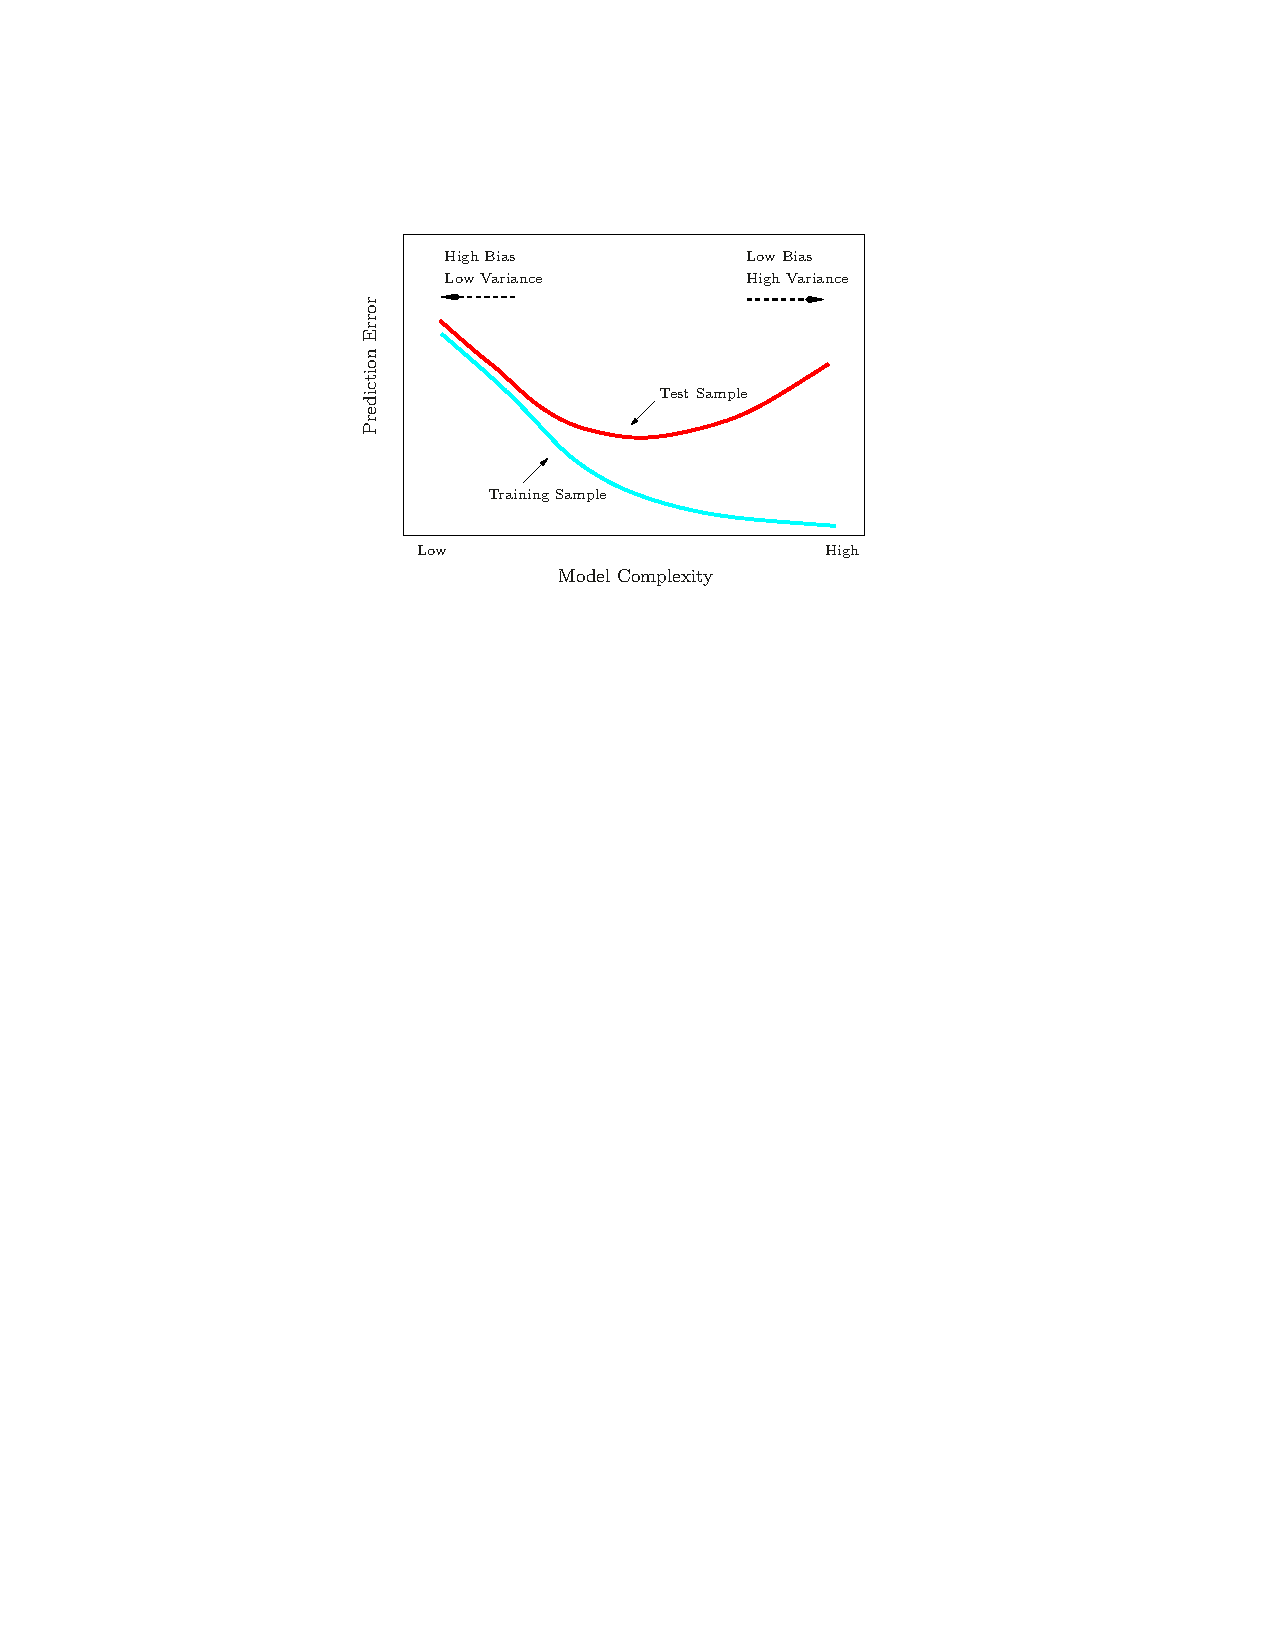
\includegraphics[width=0.8\textwidth]{figures/ml/test_train_err_curves.pdf}
\caption{
Illustrated effects of increasing model complexity on the error rates for the test and train sets \cite{HastieTF09}.
Early stopping would halt the training process when the test (or better yet, validation) set error stops decreasing.
This is also another example of the bias-variance tradeoff in action.
}
\label{fig:additional:ml:general:early_stopping}
\end{figure}

%%%%%%%%%%%%%%%%%%%%%%%%%%%%%%%%%%%%%%%%%%%%%%%%%%%%%%%%
\subsection{Silhouette Value}
\label{additional:ml:general:silhouette}
% TODO

%%%%%%%%%%%%%%%%%%%%%%%%%%%%%%%%%%%%%%%%%%%%%%%%%%%%%%%%
\subsection{Exploration-Exploitation Tradeoff}
\label{additional:ml:general:EE_tradeoff}
% TODO
 
\subsubsection{Bayesian Bandits}
\label{additional:ml:general:EE_tradeoff:BB}
% TODO
